\documentclass[11pt,a4paper]{article}
\usepackage[utf8]{inputenc}
\usepackage[ngerman]{babel}
\usepackage{subfigure} 
\usepackage{floatflt}
\usepackage{float}
\usepackage{graphicx}
\usepackage[left=3cm,right=3cm,top=3cm,bottom=3cm]{geometry}
\usepackage{natbib}
\usepackage{wrapfig}
\usepackage{listings}
\usepackage{hyperref}

\title{Robotic Games Sommersemester 2019\\ Implementierung eines Katze und Maus Spiels\\ Nachtrag}
\author{Tobias~Bak}

\begin{document}
\maketitle
\section{Problemstellung}
\begin{wrapfigure}{r}{7cm}
\centering
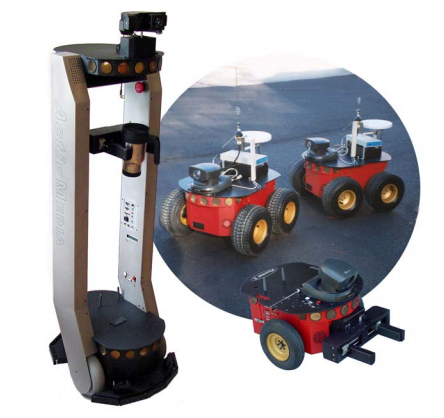
\includegraphics[scale=0.45]{media/titelbild.png}
\caption{Pioneer 3 \cite{pioneer} }
\end{wrapfigure}
Dieses Dokument enthält einen Nachtrag zur Implementierung des Katze und Maus Spiels mit dem Pioneer 3 Roboter.\cite{pioneer}

Als Aufgabe wurde an eine Gruppe von vier Personen die Anforderung den Pioneer Roboter so zu Programmieren dass dieser autonom dieses Spiel spielt. Meine Gruppe hatte die Aufgabe sehr einfach gelöst ohne Verhaltensfusion und ohne reaktiven Verhalten auf die Umgebung. Das Bedeutet der Roboter der unsere Gruppe Programmiert hatte konnte nur hinter einen Vorhang raus und zum Ziel fahren. Die Einfache Implementierung hatte großen Vorteil bei dem Spiel und gewann dieses auch mit Abstand jedoch wurde die Aufgabe nicht in der richtigen Weise gelöst. Dieses simples Verhalten ist für die Randbedingungen von Vorteil somit beschäftigt sich dieser Text mit der einer möglichst eleganten und effektiven Implementierung einer Maus die der Katze auf ihren weg ausweicht, sich versteckt und den Käse einsammelt. 

Es wird angenommen das die Maus niemals stehen bleibt. Weil die Maus immer in Bewegung bleibt und so schnell wie erlaubt Fährt ist, soll die Maus der Katze auf ihren weg frühzeitig ausweichen und falls ein Versteck in der Nähe ist erst durch das Versteck und dann zum Käse fahren. Dieses Verhalten benötigt drei Module: Vision, Fusion, Ultraschall. Wobei das Fusionsmodul ein elegantes zum Ziel Fahren und Kollisionsvermeidung beinhaltet. \\\\
Die Genaue Implementierung der Module wird nachfolgend vorgestellt.
\newpage
\section{Ultraschall}
Das Ultraschallmodul ist zunächst für das Lesen der Ultraschallsensoren zuständig. Aus gelesenen Ultraschalldaten wird eine Position eines zu vermeidendes Objekts für die Verhaltensfusion veröffentlicht. Zusätzlich wird in diesen Modul die Kollisionsvermeidung für das Versteckt ausgeschaltet. Das Modul bindet also nur die Ultraschallsensoren in das Programm ein und berechnet in welchen Winkel sich die kleinste gelesene Distanz befindet und gibt die Entfernung und den Winkel aus. 

Sei $d_o(\alpha)$ die berechnete Distanz vom Sensor der mit dem Winkel $\alpha$ am Roboter ausgerichtet ist. Weiter sei $d_i(\alpha)$ ein zweidimensionaler Vektor mit den gelesenen Daten am Sensor mit dem Winkel $\alpha$, welcher sich aus der Punktewolken Darstellung der Sensordaten ergibt. Weiter sei $d_v$ ein Vektor mit den Entfernungen zum Vorhang, dann sind die Ausgabe Distanzen wie folgt definiert:    
\begin{equation}
d_o(\alpha)=\sqrt{d_i(\alpha)_x^2+d_i(\alpha)_y^2}\cdot 2\cdot(\frac{1}{1+e^{-min(d_v)}}-0,5)
\end{equation}
Anschließend wird der Kleinste Abstand in $d_o$ gesucht und mit dem zugehörigen Winkel zusammen ausgegeben abschließend durch die Verhaltensfusion weiter verarbeitet. Der Code hierfür sieht wie folgt aus:
  
\begin{scriptsize}
\begin{lstlisting} 
#!/usr/bin/env python
import numpy as np
import rospy
from sensor_msgs.msg import PointCloud
from geometry_msgs.msg import Point
max_distance = 1
weight       = np.array([  0.5,   0.7,   1.0,   1.0,  1.0,  1.0,  0.7,  0.5])
sonar_angles = np.array(
[-90.0, -50.0, -30.0, -10.0, 10.0, 30.0, 50.0, 90.0])/ 360.0 * 2 * np.pi
class Sonar:
    def __init__(self):
        self.hideout = np.zeros(2)
        obst_sub  = rospy.Subscriber("/RosAria/sonar",PointCloud,self.sonar_callback)
        blue_sub  = rospy.Subscriber("blue_position",Point,self.hideout_callback,0)
        orang_sub = rospy.Subscriber("orange_position",Point,self.hideout_callback,1)
        while not rospy.is_shutdown():
            print("still working")
    def hideout_callback(self,data,i):
        if data.x != 0:
            self.hideout[i] = data.x
        else:
            self.hideout[i] = 100000
    def sonar_callback(self,data):
        pub       = rospy.Publisher("obstacle_position",Point,queue_size=1)
        sonar_points = data.points
        sonar_ranges = np.zeros(len(sonar_angles))
        for i in range(0, len(sonar_angles)):
            sonar_ranges[i]=np.sqrt(sonar_points[i].x**2+sonar_points[i].y**2)*2*
            (1/(1+np.exp(-1*(min(self.hideout))))-0.5)
        minimum  = np.argmin(sonar_ranges)
        output   = Point()
        if sonar_ranges[minimum] <= max_distance:
            output.x = sonar_ranges[minimum]*weight[minimum]
            output.y = -sonar_angles[minimum]
        pub.publish(output)
if __name__== '__main__':
    rospy.init_node("obstacle_detection")
    try:
        node=Sonar()
    except rospy.ROSInterruptException:
        rospy.loginfo("sonar not working")
\end{lstlisting} 

\end{scriptsize}
\newpage
\section{Vision}      
Die Vision ist das Modul um Objekte per Kamera zu erkennen. Es wurde während dieses Projekts nach Farben selektiert, so waren die Katzen Rot, die Vorhänge Gelb und Blau und der Käse Grün. Das Vision Modul sucht abhängig von gewählten Farbe nach Objekten dieser Farbe und Gibt die Entfernung und den Winkel des Objekts aus welchen von der Verhaltensfusion weiter verarbeitet werden.

 Im Ablauf ist das Modul wie folgt aufgebaut. Zunächst wird das Bild in den HSV Farbraum konvertiert anschließend werden über das Bild zwei Masken gelegt. Eine Maske schneidet den obere Bildhälfte ab die andere Maske blendet alle Farben die in nicht definierten Raum befinden aus. So vorbereitetes Bild wird nach Konturen durchgesucht. In den Konturen selbst wird die größte Kontur gesucht und eine Box um diese gelegt. Aus den Maßen der Box werden anschließend der Winkel $\alpha$ und die Entfernung $d$ berechnet. Wobei $f$ die Fokuslänge, $x,y$ die Position des Pixels am weitesten links oben und $w,h$ die Breite und die Höhe des Objekts sind sowie $img_w$ die Gesamtbreite des Bildes ist. Damit ergibt sich für den Winkel $\alpha$:
\begin{equation}
\alpha = -\arctan(\frac{(x+w\cdot 0,5-\frac{img_w}{2})}{f})
\end{equation}   
und für die Entfernung:
\begin{equation}
d=\frac{f}{h*\cos(\alpha)}
\end{equation}
Der Code hierfür sieht wie folgt aus:
\begin{tiny}
\begin{lstlisting}
#!/usr/bin/env python
import sys
import cv2
import rospy
from sensor_msgs.msg import Image
from geometry_msgs.msg import Point
from cv_bridge import CvBridge
import numpy as np
focal_len        = 500
min_size         = 600
max_height       = 200
global last_cheese
last_cheese      = 0
def img_call(ros_img):
	global last_cheese
	cv_img                   = bridge.imgmsg_to_cv2(ros_img,'rgb8')
	image_h, image_w         = cv_img.shape[:2]
	hsv_img                  = cv2.cvtColor(cv_img, cv2.COLOR_RGB2HSV)
	mask                     = cv2.inRange(hsv_img,np.array([int(sys.argv[3]),int(sys.argv[4]),
	int(sys.argv[5])]) , np.array([int(sys.argv[6]),int(sys.argv[7]),int(sys.argv[8])]) )
	mask                     = cv2.rectangle(mask,(0,0),(len(mask[0]),max_height),(0,100,0),-1)
	im2, contours, hierarchy = cv2.findContours(mask, cv2.RETR_EXTERNAL, cv2.CHAIN_APPROX_SIMPLE)
	output                   = Point()
        if int(sys.argv[9]) == 1:
            output.x                 = 1
            output.y                 = last_cheese
	if len(contours) > 0:
		biggest_contour=max(contours, key = cv2.contourArea)
		if cv2.contourArea(biggest_contour) >= min_size:
			x,y,w,h         = cv2.boundingRect(biggest_contour[0])
			output.y            = -1*np.arctan((x+w*0.5-image_w/2.0)/focal_len)
			output.x            = float(sys.argv[2])*focal_len/(h*np.cos(output.y))
			last_cheese         = output.y
	pubCheese.publish(output)
if __name__ == '__main__':
	try:
		rospy.init_node("vision")
                bridge       = CvBridge()
		cam_sub      = rospy.Subscriber('/usb_cam/image_raw',Image,img_call)
                pubCheese    = rospy.Publisher(sys.argv[1], Point, queue_size=1)
		rospy.spin()
	except rospy.ROSInterruptException:
		rospy.loginfo("vision type node not working")

\end{lstlisting}

\end{tiny}
\newpage
\section{Fusion}
Das Fusionsmodul übernimmt mehrere Aufgaben. Zunächst ist es für das Starten des Zuhörens auf verschiedene Instanzen der Vision und . So wird die Vision vorher mit verschiedenen Farben für verschiedene Objekte und das Ultraschallmodul gestartet und drauf gehört. Anschließend werden alle Daten eingesammelt und zur resultierenden Bewegungskommando berechnet und an den Roboter gesendet. Für die eigentliche Verhaltensfusion wurden Analogical Gates\cite{gates} implementiert und wie in der \autoref{gates} verschaltet. 
\begin{figure}[H]
\centering
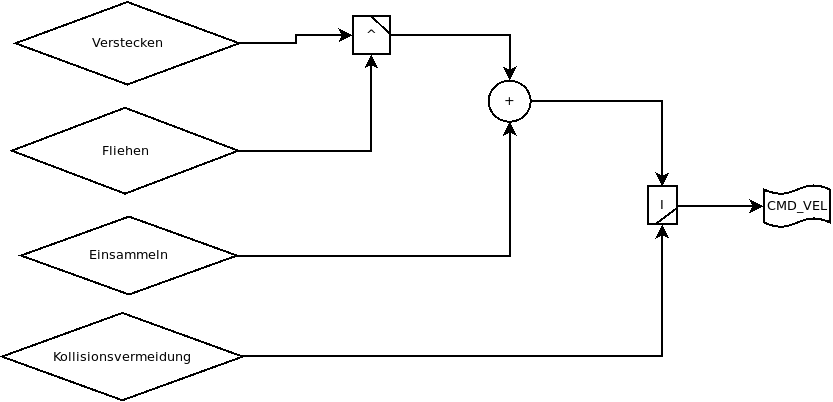
\includegraphics[scale=0.5]{media/gates.png}
\caption{Analogical Gates}\label{gates}
\end{figure}
Die Verhalten in der \autoref{gates} sind wie Folgt definiert. Das Verstecken hat als Input die Position des Verstecks. Wenn die Position des Verstecks günstig ist soll sich versteckt werden. Fliehen schaltet sich ein wenn die Katze im Bild zu sehen ist und es wird die Katze vermieden indem die Katze aus dem Rand des Bildes verschwindet. Das Einsammeln des Käses funktioniert umgekehrt zu Vermeidung der Katze und zwar wird hier versucht den Käse in die Mitte des Bildes zu kriegen. Kollisionsvermeidung ist immer bis auf Versteck eingeschaltet und wird als meist bevorzugtes Verhalten durchgeschaltet. 

So konsturietes Programm folgt in der \autoref{rnbc} gezeigten Struktur. Es ist keine RNBC (Recursive Nested Behaviour Control) \cite{rnbc} Struktur auf Grund der Wiederverwendung des geschrieben Codes und um die Implementierung elegant gestalten zu können.    
\begin{figure}[H]
\centering
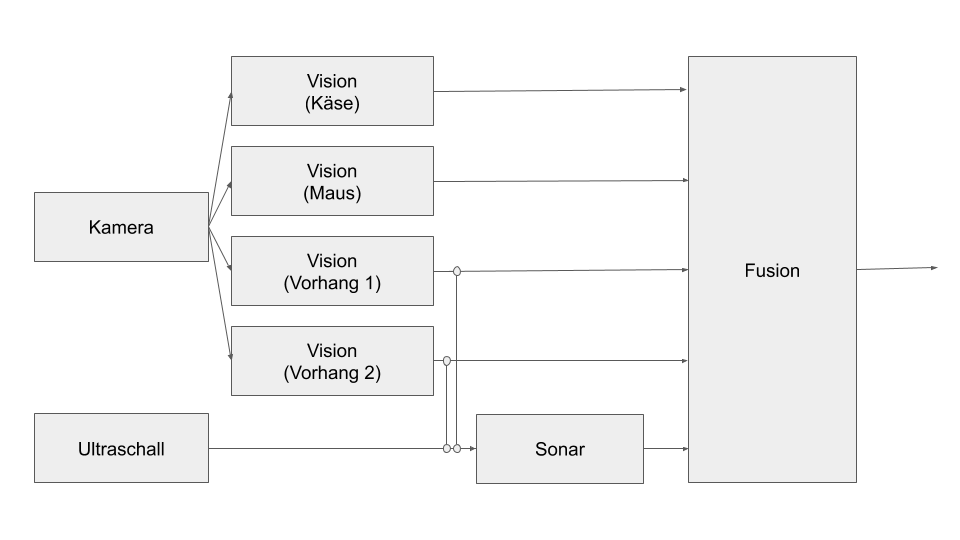
\includegraphics[scale=0.7]{media/struktur.png}
\caption{Programmstruktur}\label{rnbc}
\end{figure}
Die Genaue Implementierung sieht wie folgt aus:
\begin{tiny}
\begin{lstlisting}
#!/usr/bin/env python
import sys
import rospy
import numpy as np
from geometry_msgs.msg import Twist
from geometry_msgs.msg import Point
class Fusion:
	def __init__(self):
                # array containes cat,blue,orange,cheese,collision
                self.behaviors = np.zeros((5,2))
                parameters     =  np.array([[-0.5,-1,-1],[0.3,0,1],[0,0,1],[0.8,0,1],[-0.5,-1,-1]])
                for i in range(5):
                    rospy.Subscriber(sys.argv[i+1], Point, self.generate_behavior,
                    (i,parameters[i,0],parameters[i,1],parameters[i,2]))
		self.pub                     = rospy.Publisher('/RosAria/cmd_vel', Twist, queue_size=1)
		while not rospy.is_shutdown():
			self.fusion()
        def generate_behavior(self,msg,args):
                print(args[0])
                if msg.x != 0 and msg.y != 0 :
                    self.behaviors[args[0]] = np.array([1,args[1]*msg.x**args[2]*msg.y**args[3]])
                else:
                    self.behaviors[args[0]] = np.array([1,0])

	def fusion(self):
		#print('collision', self.collision, 'cheese', self.cheese)
		cmd_vel = Twist()
		cmd_vel.linear.x = 1
                cmd_vel.angular.z = prevail_gate(or_gate(
                invoke_gate(self.behaviors[2,1],self.behaviors[0,1]),self.behaviors[3,1]),self.behaviors[4,1])
                #cmd_vel.angular.z = self.behaviors[1,1]
                print(self.behaviors)
		self.pub.publish(cmd_vel)
def and_gate(x, y):
        a = 2.28466
        b = -0.89817
        if x == 0 and y == 0:
            return 0
        else:
            return x*(1-np.exp(-((a*y**2+b*x*y)/(x**2+y**2))))+ y*(np.exp(-((a*x**2+b*x*y)/(x**2+y**2))))
def or_gate(x, y):
        a = 1.02889
        b = 0.3574
        if x == 0 and y == 0:
            return 0
        else:
            return x*(np.exp(-((a*y**2+b*x*y)/(x**2+y**2)))) + y*(np.exp(-((a*x**2+b*x*y)/(x**2+y**2))))
def invoke_gate(x, y):
        return and_gate(or_gate(x, y),x)
def prevail_gate(x, y):
        return or_gate(x, or_gate(x, y))
if __name__ == '__main__':
	try:
		rospy.init_node("fusion")
		fus = Fusion()	
	except rospy.ROSInterruptException:
		rospy.loginfo("---------- FUSION-ERROR! ---------")
\end{lstlisting}
\end{tiny}
%\bigskip\bigskip\bigskip\bigskip\bigskip\bigskip\bigskip\bigskip
%Diese Arbeit entstand mit Hilfe von B.Sc. Jan Baumgärtner, vielen dank dafür.
\newpage
% Festlegung Art der Zitierung - Havardmethode: Abkuerzung Autor + Jahr
\bibliography{lit}
\bibliographystyle{abbrv}
\end{document}